
\documentclass[a4paper]{report}

\usepackage[utf8]{inputenc}
\usepackage[english]{babel}
\usepackage[T1]{fontenc}
\usepackage{textcomp}
\usepackage[]{amsthm} 
\usepackage[]{amssymb}
\usepackage{graphicx}
\usepackage{float}
\usepackage{soul}
\usepackage{color}
\usepackage{bm}
\usepackage{listings}
\usepackage{xcolor}
\usepackage{enumitem}
%\usepackage{xfrac}
\usepackage[normalem]{ulem}

% ~~~~ fancy symbol ~~~~
\usepackage{bbding}

% ~~~~ no indent per paragraph ~~~~-
\usepackage[parfill]{parskip}

% ~~~~ hyperlinks ~~~~ 
\usepackage[colorlinks=true, linkcolor=blue]{hyperref}

% ~~~~ subfigs ~~~~
\usepackage{subcaption}

% ~~~~ math ~~~~
\usepackage{amsmath}

% ~~~~ .prt files ~~~~
\usepackage{fancyvrb}

\usepackage{mathtools}
% ~~ colorbox : "align" use only ~~
\newcommand{\myboxA}[1]{
	\fcolorbox{black}{lime}{#1}
}
\MakeAboxedCommand\AboxedA\myboxA

% ~~ colorbox : else ~~
\newcommand{\mybox}[1]{
	\fcolorbox{black}{lime}{$\displaystyle#1$}
}

% ~~~~ graphics ~~~~
\usepackage{tikz}
\usetikzlibrary{trees}
\usetikzlibrary {fit,shapes.geometric} % W: Command terminated with space. (1)
\usetikzlibrary {automata} % W: Command terminated with space. (1)
\usetikzlibrary{arrows.meta}
\usepackage{multicol}

\usepackage{pgfplots}
\pgfplotsset{compat = newest}

\usepackage{geometry}
\geometry{legalpaper, margin=1in}

% ~~~~ upgraded tables ~~~~
\usepackage{booktabs}

% ~~~~ algorithm formatting ~~~~
\usepackage{algorithm}
\usepackage[noend]{algpseudocode}
\usepackage{caption}

% ~~~~ list bullets ~~~~
\renewcommand{\labelitemii}{$\circ$}
\renewcommand{\labelitemiii}{$\star$}
\renewcommand{\labelitemiv}{$>$}

% figure support
\usepackage{import}
\usepackage{xifthen}
\pdfminorversion=7
\usepackage{pdfpages}
\usepackage{transparent}
\newcommand{\incfig}[1]{%
    \def\svgwidth{\columnwidth}
    \import{./figures/}{#1.pdf_tex}}

% Newline for algorithm psuedo
\newcommand{\algrule}[1][.2pt]{\par\vskip.5\baselineskip\hrule height #1\par\vskip.5\baselineskip}

% -------- Listings/XColor Settings --------
\definecolor{codegreen}{rgb}{0,0.6,0}
\definecolor{codegray}{rgb}{0.5,0.5,0.5}
\definecolor{codepurple}{rgb}{0.58,0,0.82}
\definecolor{backcolour}{rgb}{0.95,0.95,0.92}

\lstdefinestyle{mystyle}{
	backgroundcolor=\color{backcolour},
	commentstyle=\color{codegreen},
	keywordstyle=\color{magenta},
	numberstyle=\tiny\color{codegray},
	stringstyle=\color{codepurple},
	basicstyle=\ttfamily\scriptsize,
	breakatwhitespace=false,
	breaklines=true,
	captionpos=b,
	keepspaces=true,
	numbers=left,
	numbersep=5pt,
	showspaces=false,
	showstringspaces=false,
	showtabs=false,
	tabsize=4
}

\lstset{style=mystyle}

% -------------- Doc Start -------------------



\pdfsuppresswarningpagegroup=1

\title{\Huge{Designing a Fibonacci Accelerator}}
\author{\textbf{Authors:} \\WhisperingRock}
\date{Class\\CPE490: Open-Source ASIC Design\\\today}

\begin{document}
    \maketitle
	
	% ~~~~ add toc as a bookmark ~~~~
	\phantomsection
	\addcontentsline{toc}{section}{\contentsname}

	\tableofcontents

	\chapter{Introductions}
		In this lab, the task was to create a Fibonacci accelerator. Before
		going further in the paper, I must first describe the Fibonacci 
		sequence and what makes a design an \textit{accelerator}. 

		First, let's discuss the Fibonacci sequence using a recursive formula. 
		\[
			\bm{F_{n+2} = F_{n+1} + F_{n} \text{ where } F_0 = 0 \text{ and } F_1 = 1}
		\]

		In our discussion in class, another relationship emerged when comparing multiple terms.

		Consider:
		\begin{itemize}
			\item Let $F_{n} = a$ 
			\item Let $F_{n+1} = b$ 
			\item $F_{n+2} = a + b$
			\item $F_{n+3} = a + 2b$
			\item $F_{n+4} = 2a + 3b$
			\item $F_{n+5} = 3a + 5b$
		\end{itemize}

		If given two terms of the sequence, we can potentially calculate
		the next four terms from the initial two. This unique way to describe terms 
		has potential for a speed-up if we can utilize shifters and adders
		with the motivation to calculate many terms in a single cycle. 

		This motivation to increase throughput or performance over a CPU, 
		through the use of configurable logic, is termed as an \textit{accelerator}. 
		For this lab, our accelerator will calculate more than one term
		of the Fibonacci sequence per clock cycle. 

		Lastly, another motivation of this lab is to become familiar with 
		open-source tooling set. 

	\chapter{v0 Pre-Synthesis}

		\section{Procedure}
			The workflow of this lab, which is largely focused on design before
			synthesis, will be the following

			\begin{enumerate}
				\item LINTing based off of many tools s.a. Verilator, Icarus, GL, \ldots
				\item Simulation of test scripts on Verilator, then Icarus Verilog
				\item BMC verification 
				\item \textit{K}-Induction formal verification (optional)
			\end{enumerate}

		\section{Design}

			\begin{figure}[H]
				\centering
				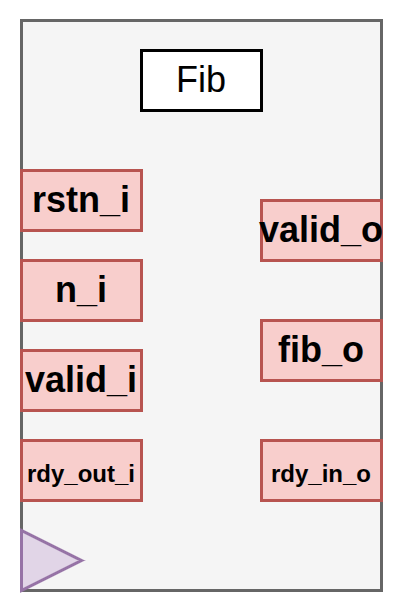
\includegraphics[
					width			= 0.3\textwidth,
					keepaspectratio	= true
				]{./version0/top.png}
				\label{fig:top}
				\caption{Fibonacci Top Module}
			\end{figure}

			The top-level module has a data and control signals:
			\begin{itemize}
				\item \textbf{clk\_i}: clock (posedge is captured).
				\item \textbf{rstn\_i}: active-low synchronous reset.
				\item \textbf{valid\_i}: indicates when input n\_i can be read.
				\item \textbf{n\_i}: requested term of fib sequence.
				\item \textbf{rdy\_out\_i}: indicates when downstream has read this modules output
					(and module can begin processing a new sequence).\\
				\item \textbf{valid\_o}: indicates module's output is ready to be read.
				\item \textbf{rdy\_on\_o}: indicates module is ready for a new request (n\_i).
				\item \textbf{fib\_o}: modules output ($F_{n}$).
			\end{itemize}


			In order to capture the functionality of these top-level signals, 
			an FSM was used:

			\begin{figure}[H]
				\centering
				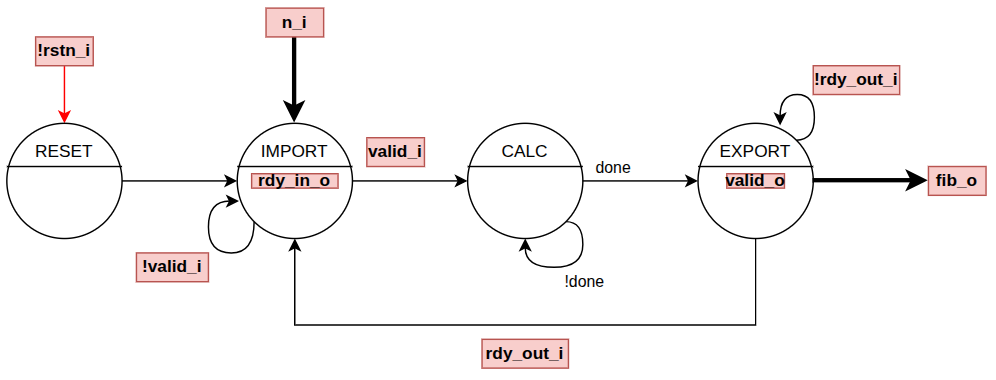
\includegraphics[
					width			= 0.8\textwidth,
					keepaspectratio	= true
				]{./version0/fsm.png}
				\caption{FSM of Fibonacci Accelerator}
				\label{fig:fsm}
			\end{figure}

			From here, lets take a closer look into the CALC stage of the FSM, where most
			of our accelerator logic comes into play. An attentive reader will notice that there 
			are only two adders and a single shifter: there is a considerable 
			amount of adders required to further calculate $F_{n+4}$ and $F_{n+5}$.
			Since this must be implemented in ASIC where wires and hardware are not
			free lunches, this designer opted to take 2 cycles to calculate 4 terms 
			of the fib sequence. This will keep the area smaller while producing
			two elements per cycle (a +2x increase over a CPU).

			\begin{figure}[H]
				\centering
				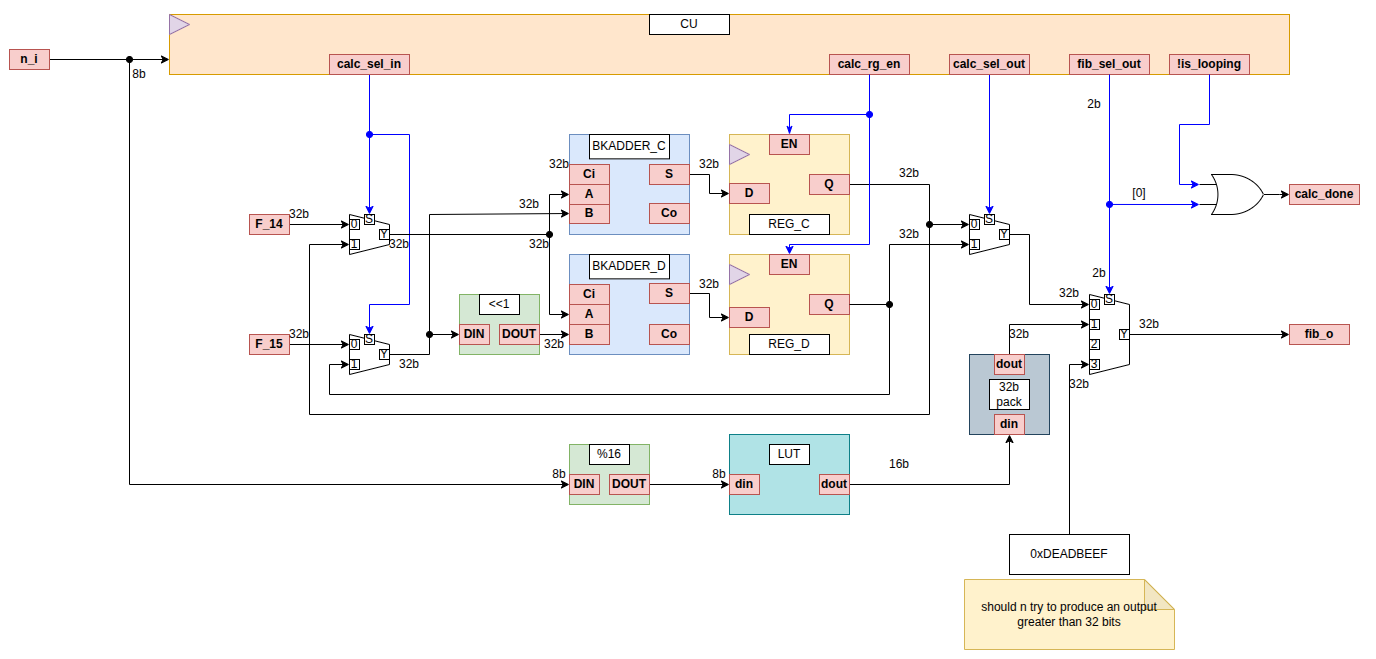
\includegraphics[
					width			= \textwidth,
					keepaspectratio	= true
				]{./version0/accelerator.png}
				\caption{Computation Portion of Fib Accelerator}
				\label{fig:comp}
			\end{figure}

			\begin{figure}[H]
				\centering
				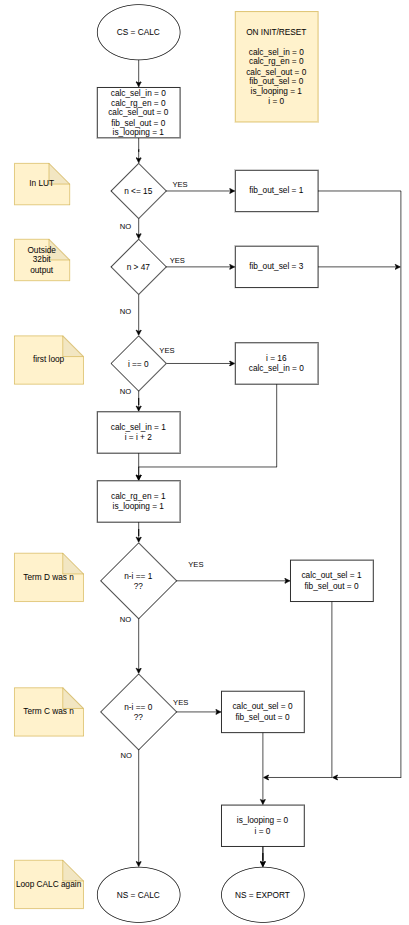
\includegraphics[
					width			= 0.4\textwidth,
					keepaspectratio	= true
				]{./version0/calc_flow.png}
				\caption{Control Flow of CALC State}
				\label{fig:calcflow}
			\end{figure}

			To properly explain the design, let's trace through various values 
			of $n$.

			\begin{figure}[H]
				\centering
				\begin{subfigure}[t][][b]{\textwidth}
					\centering
					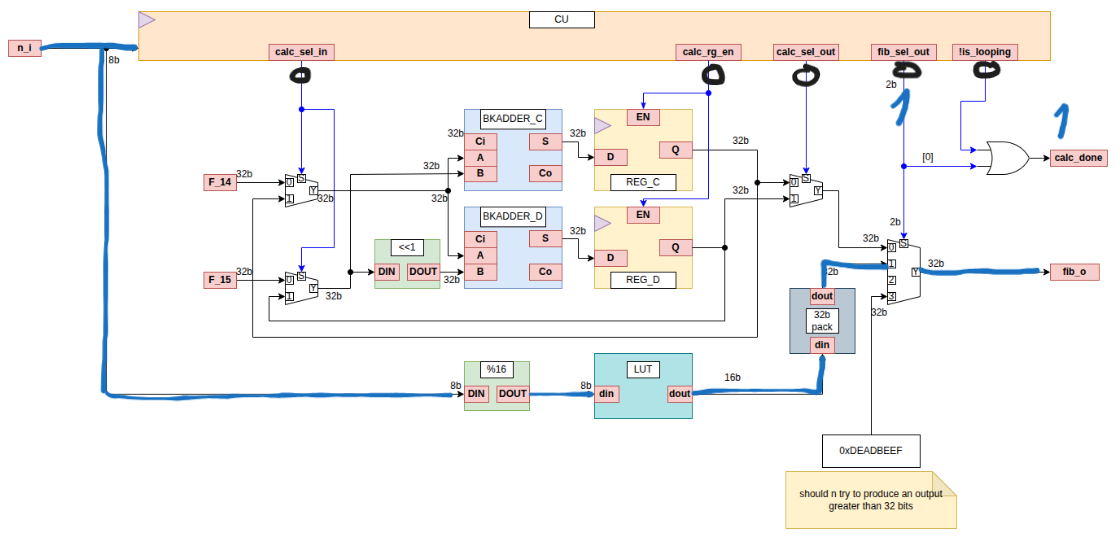
\includegraphics[
						width			= 1.0\textwidth,
						keepaspectratio	= true
					]{./version0/calc_flow_lowLUT.png}
				\end{subfigure}
				\begin{subfigure}[t][][b]{\textwidth}
					\centering
					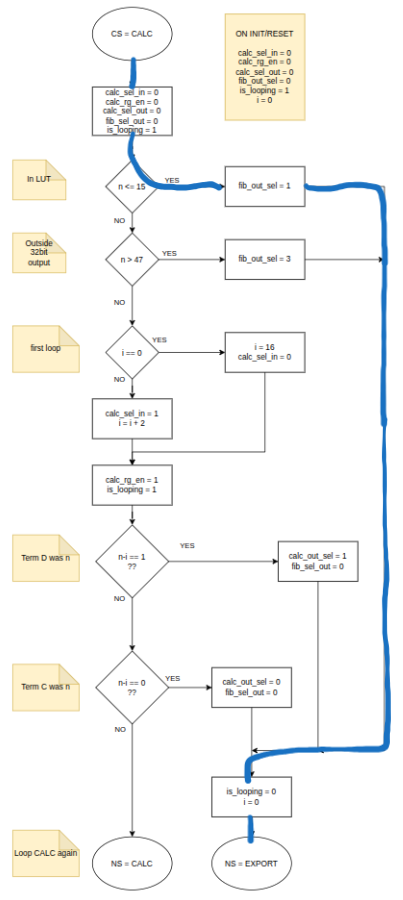
\includegraphics[
						width			= 0.5\textwidth,
						keepaspectratio	= true
					]{./version0/calc_flow_lowLUT1.png}
				\end{subfigure}
				\caption{$n \le 15$ uses the LUT}
				\label{fig:lowlut}
			\end{figure}

			\begin{figure}[H]
				\centering
				\begin{subfigure}[t][][b]{\textwidth}
					\centering
					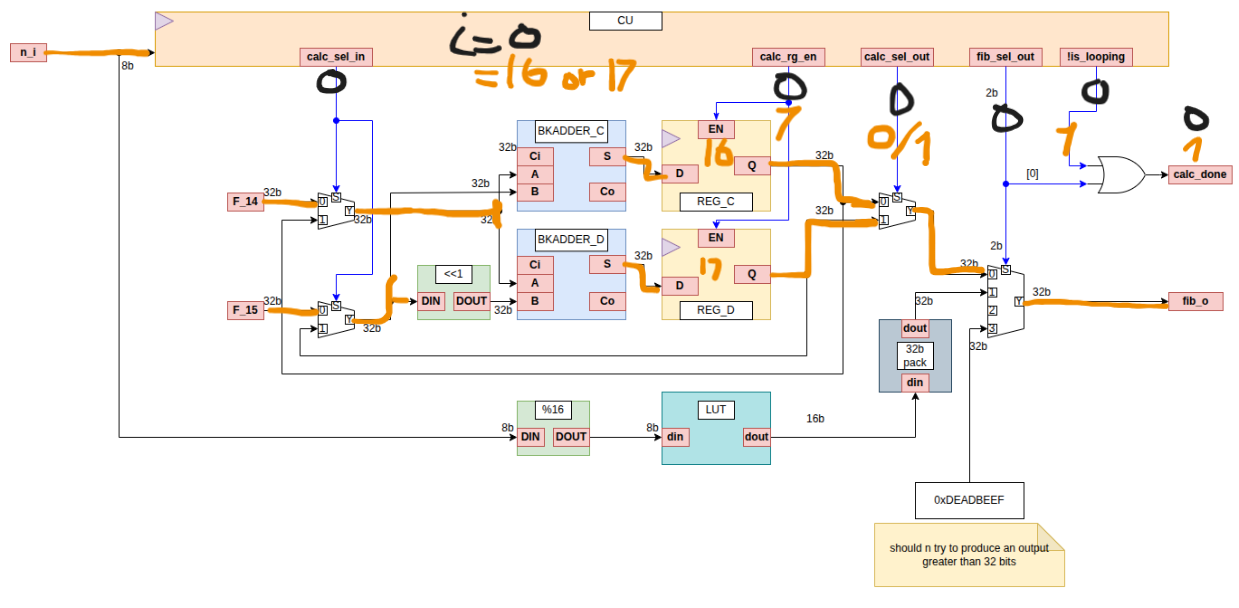
\includegraphics[
						width			= 1.0\textwidth,
						keepaspectratio	= true
					]{./version0/calc_flow_first.png}
				\end{subfigure}
				\begin{subfigure}[t][][b]{\textwidth}
					\centering
					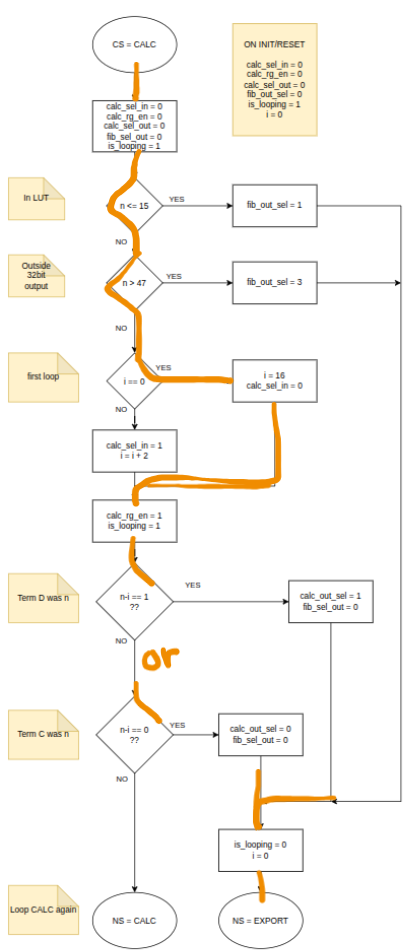
\includegraphics[
						width			= 0.5\textwidth,
						keepaspectratio	= true
					]{./version0/calc_flow_first1.png}
				\end{subfigure}
				\caption{$n = 16$ or $n=17$ calculates but doesn't loop}
				\label{fig:firstcalc}
			\end{figure}

			\begin{figure}[H]
				\centering
				\begin{subfigure}[t][][b]{\textwidth}
					\centering
					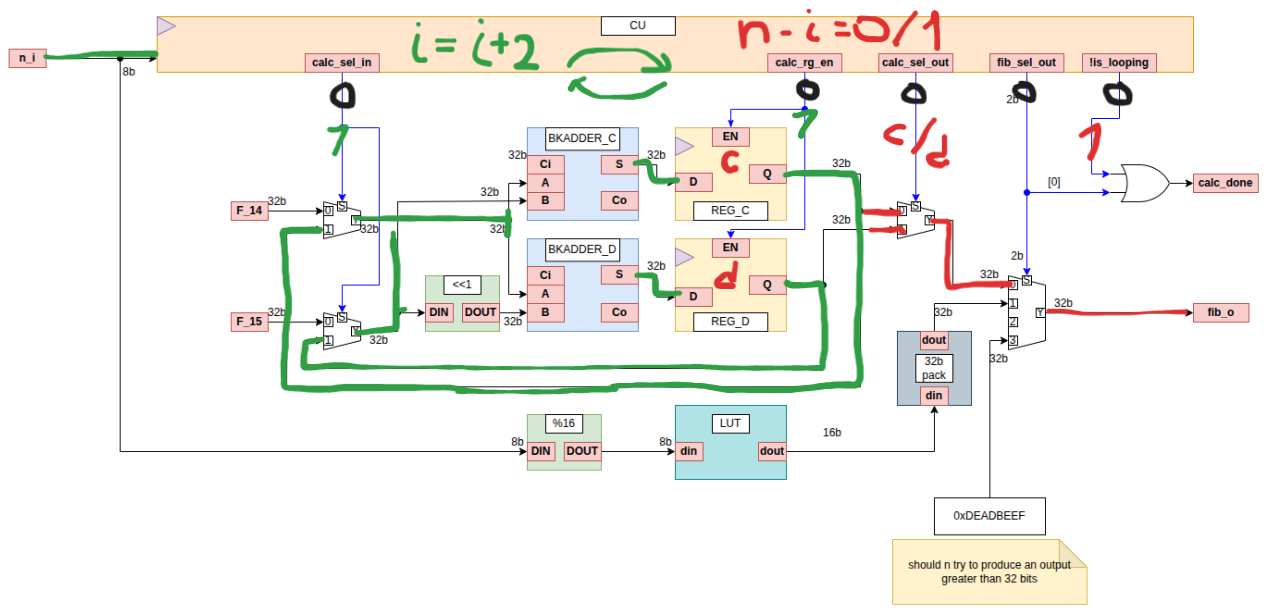
\includegraphics[
						width			= 1.0\textwidth,
						keepaspectratio	= true
					]{./version0/calc_flow_ongoing.png}
				\end{subfigure}
				\begin{subfigure}[t][][b]{\textwidth}
					\centering
					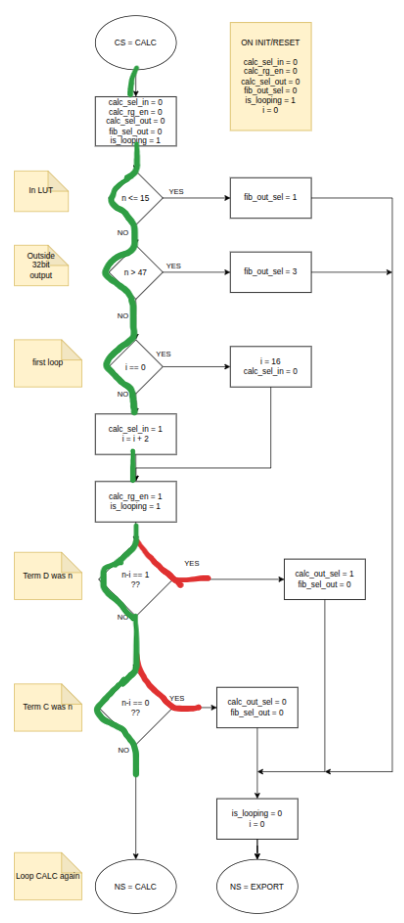
\includegraphics[
						width			= 0.5\textwidth,
						keepaspectratio	= true
					]{./version0/calc_flow_ongoing1.png}
				\end{subfigure}
				\caption{$n \ge 18$ and $n \le 47$ calculates using loops}
				\label{fig:loopcalc}
			\end{figure}

			\begin{figure}[H]
				\centering
				\begin{subfigure}[t][][b]{\textwidth}
					\centering
					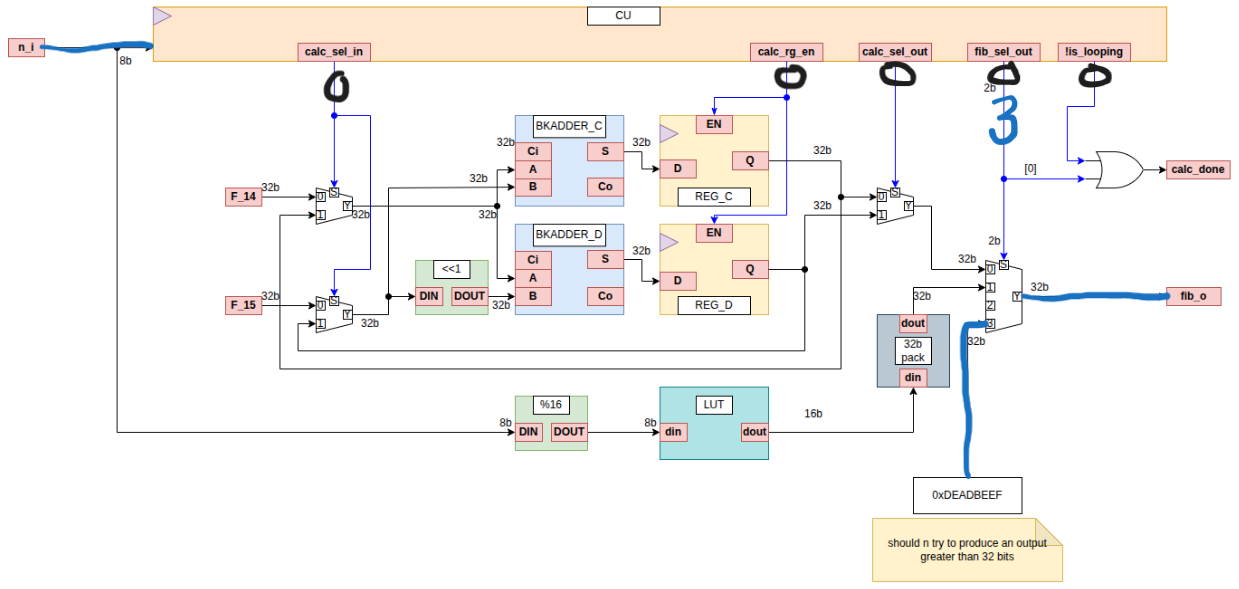
\includegraphics[
						width			= 1.0\textwidth,
						keepaspectratio	= true
					]{./version0/calc_flow_highLUT.png}
				\end{subfigure}
				\begin{subfigure}[t][][b]{\textwidth}
					\centering
					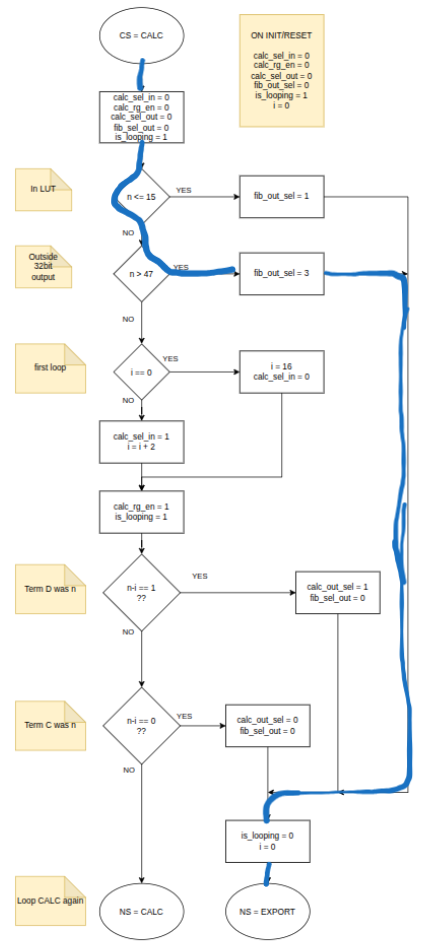
\includegraphics[
						width			= 0.5\textwidth,
						keepaspectratio	= true
					]{./version0/calc_flow_highLUT1.png}
				\end{subfigure}
				\caption{$n > 47$ defaults to avoid output overflow}
				\label{fig:loopceil}
			\end{figure}

		\section{Simulation Testing}

			\subsection{Brent-Kung `Parallel Prefix' Adder}
				The BKAdder was studied and implemented as a dynamic model, only verified
				using formal verification methods BMC and \textit{K}-Induction. The
				rtl and verification can be seen in the same file~\ref{adder}. 

				\begin{table}[H]
					\centering
					\begin{tabular}{lc}
						\toprule
						\textbf{Test Type} & \textbf{Result} \\
						\midrule
							BMC & \checkmark\\
							\midrule
							Induction & \checkmark\\
						\bottomrule
					\end{tabular}
					\caption{Verification Methods for BKAdder}
				\end{table}

			\subsection{Fibonacci Accelerator}
				The accelerator was initially verified using immediate and concurrent
				simulations on verilator (not icarus because SVA is not supported). 
				The simulation file~\ref{tb-fib} tests:

				\begin{itemize}
					\item \textbf{Concurrents}
						\begin{itemize}
							\item \textbf{reset\_import}: confirms the module comes out
								of RESET, enters the IMPORT state, and signals the upstream
								that it is ready to accept an input $n$.

							\item \textbf{import\_export}: confirms the model is not 
								holding the output steady while prompting the upstream
								for a new input $n$.

							\item \textbf{hold\_fib}: confirms the output \texttt{fib\_o} was
								steady as long as our module is finished calculating and the downstream
								has not confirmed an output read.
						\end{itemize}

					\item \textbf{Immediates}
						\begin{enumerate}
							\item Test $n \in [0,47]$ outputs the correct values sequentially.
							\item Test $n \in [48,255]$ outputs an error code because output overflow is certain.
						\end{enumerate}
				\end{itemize}

				\begin{table}[H]
					\centering
					\begin{tabular}{lc}
						\toprule
						\textbf{Test Type} & \textbf{Result} \\
						\midrule
							Verilator (SVA) Concurrents & \checkmark\\\midrule
							Verilator (SVA) Immediates& \checkmark\\\midrule
							Icarus (SVA) Immediates& \checkmark\\\midrule
							BMC & \XSolidBrush\hl{TODO}\\\midrule
							Induction & \XSolidBrush\hl{TODO}\\
						\bottomrule
					\end{tabular}
					\caption{Verification Methods for BKAdder}
				\end{table}

	\chapter{v0 Post-Synthesis Analysis}

		\lstinputlisting[
			captionpos	= top, 
			caption		= {v0 LibreLane config settings},
			breaklines	= false, 
			label		= {}
		]{./version0/config.yaml}	
		
		\section{Static Timing Analysis (Pre-PlaceNRoute)}

			\lstinputlisting[
				captionpos	= top,
				caption		= {Overall Summary of Initial Post-Layout Simulation},
				breaklines	= false, 
				label		= {sta:init-summary},
				firstline	= 1292,
				lastline	= 1310
			]{./version0/initial_flow.log}

			\lstinputlisting[
				basicstyle	=\ttfamily\tiny,
				captionpos	= top,
				caption		= {openroad-staprepnr Summary},
				breaklines	= false, 
				label		= {sta:init-prepnr}
			]{./version0/initial_staprepnr.rpt}

			After performing an initial static-timing analysis, there
			is evidence of setup violations in the pre-place and route
			phase, with the biggest offending corner at 
			\texttt{nom\_ss\_100C\_1v60}. Since this corner is testing logic
			speeds at the lowest worse case, we can infer that our logic is too slow and
			that the longest and slowest paths cannot meet out target frequency
			of 10ns. Now that we've identified which corner is the biggest thorn, 
			we can start to ask where and which path(s) are in violation. 

			NOTE: Lets reside in pre-pnr for now, since the likelihood our
			timing issues will resolve after placement is not good. 
			
			\newpage
			\lstinputlisting[
				basicstyle	=\ttfamily\tiny,
				captionpos	= top,
				caption		= {Route for Setup's Biggest Offender},
				breaklines	= false, 
				label		= {sta:init-max},
				lastline	= 74
			]{./version0/initial_max.rpt}

			Looking at fig~\ref{sta:init-max}, there are a few items that stand out.
			\begin{itemize}
				\item L25: signal \verb|fib_sel_out[0]| has a fanout of 126 when its rising ($\wedge$).
					Moreover, we occurred a massive delay and skew on this one transaction. 
				\item L27-59: The end bits on the input mux b are DOWNSTREAM 
					and ADDING to the delay of this path. 
			\end{itemize}

			\subsection{Analysis}

				\begin{itemize}
					\item Q: Why is there such a large fanout on this signal?
						This signal is the SEL signal for the \verb|mux_fib| in 
							fig~\ref{fig:comp}, meaning that it is connected to many 
							smaller muxes to drive the 128-bit one. This, on the surface, doesn't
							sound too problematic if this was the only logic to be calculated. Might
							there be something else wrong?
							
					\item Lets scrutinize the path in fig~\ref{fig:loopcalc} as
						I suspect its also causing unnecessary delay. First, lets outline
						what is actually happening here, assuming a newly
						calculated term is our requested one (b/c its worst case). 

						\begin{enumerate}
							\item While the CU flies through the conditional statements, 
								the adders are beginning to calculate new terms
								for C and D. 
							\item Register enable is high s.t.\ we capture these
								calculations.
							\item We configure \textbf{two} 32-bit muxes to deliver
								term D to \verb|fib_o| as well as set \verb|calc_done|.
							\item The adders finish and the registers capture. 
							\item The output muxes receive the data on the next
								clock cycle.
						\end{enumerate}

						The initial inspiration was to store the new calculations in 
						the registers as well as config the muxes, then by the EXPORT
						stage, we should hold and be ready to output the correct value. 
						Unfortunately, this is too much logic to run through in a single
						stage and clock cycle. Moreover, a second 32-bit mux on the 
						output is not needed. 
				\end{itemize}

			\newpage
			\chapter{v1 Redesign + Analysis}

				\begin{figure}[H]
					\centering
					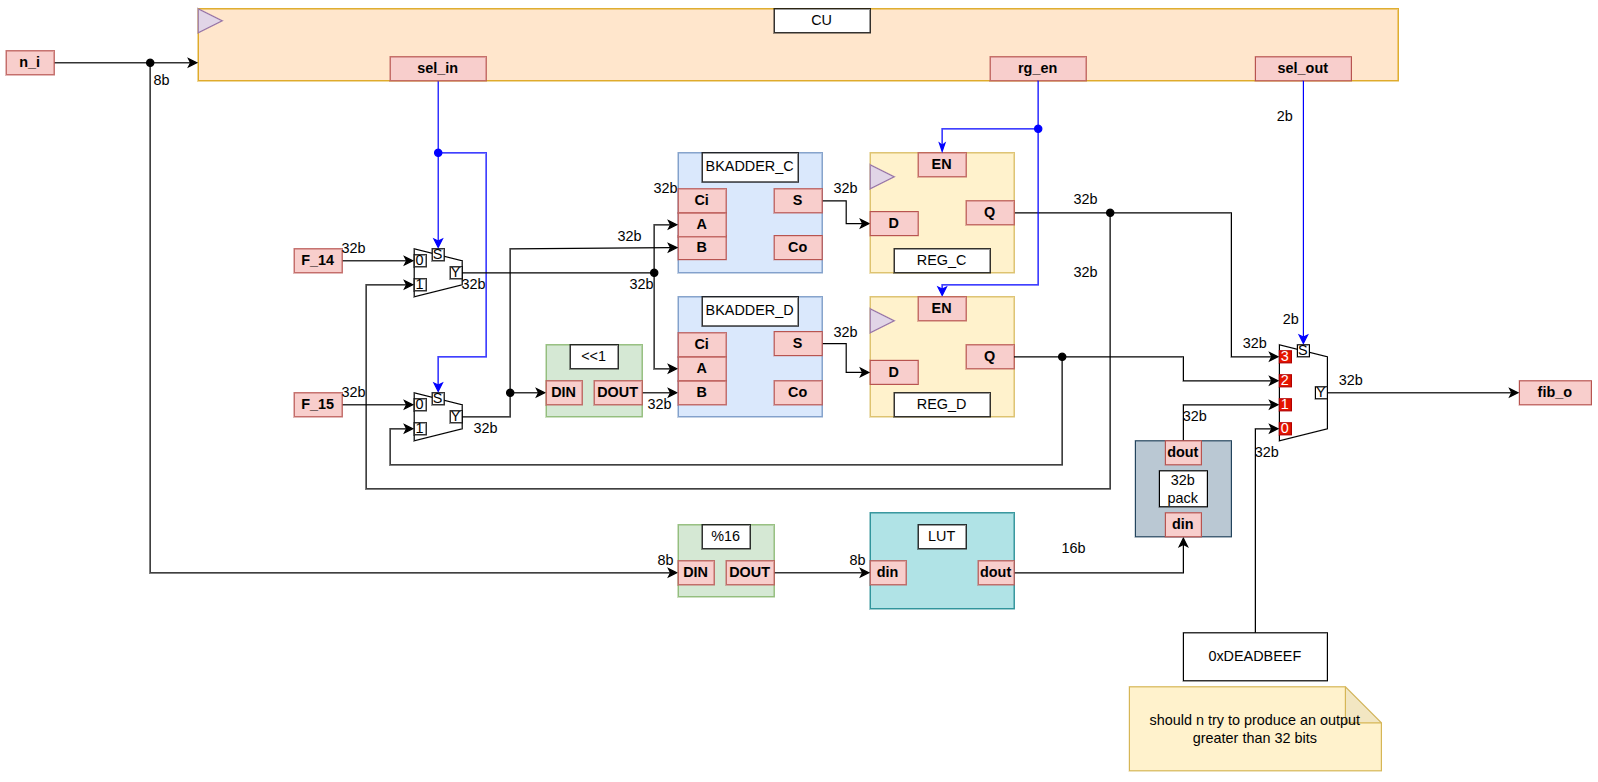
\includegraphics[
						width			= 0.9\textwidth,
						keepaspectratio	= true
					]{./version1/accelerator.png}
					\caption{v1 Accelerator Logic}
					\label{fig:v1-acc}
				\end{figure}

				\begin{figure}[H]
					\centering
					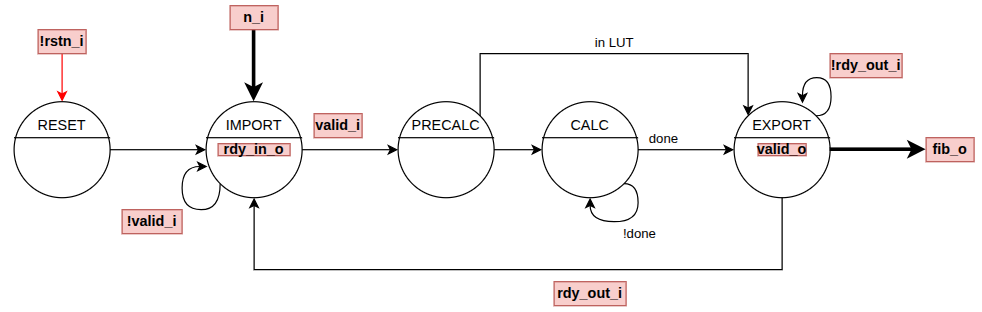
\includegraphics[
						width			= 0.6\textwidth,
						keepaspectratio	= true
					]{./version1/fsm.png}
					\caption{v1 Accelerator FSM}
					\label{fig:v1-fsm}
				\end{figure}

				\begin{figure}[H]
					\centering
					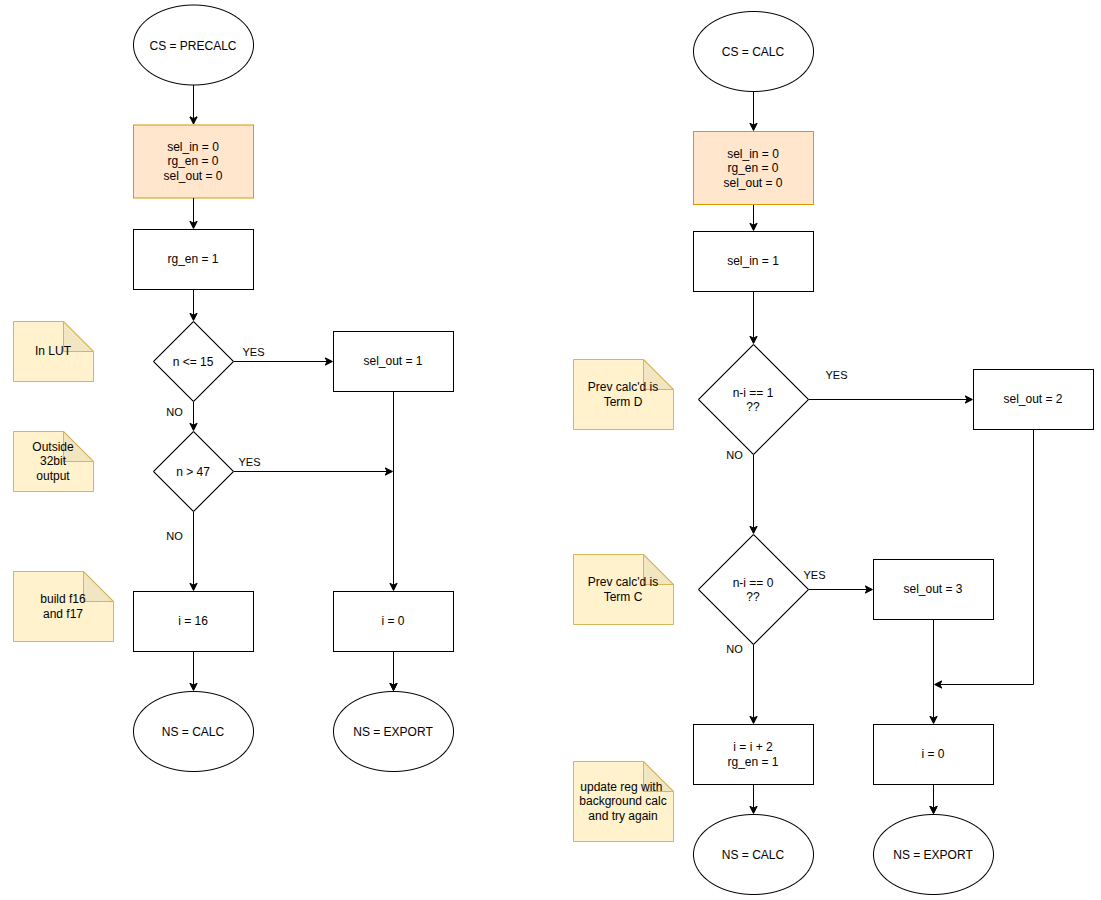
\includegraphics[
						width			= 0.6\textwidth,
						keepaspectratio	= true
					]{./version1/flow.png}
					\caption{v1 Accelerator Flow}
					\label{fig:v1-flow}
				\end{figure}
				
				\newpage
				This redesign 
				\begin{itemize}
					\item Removed an output 2-Mux and wired the registers
						directly to the output mux.
					\item Removed the \verb|calc_done| logic and based
						the state logic around CU's internal signals.
					\item Broke up \verb|CALC| logic into two states \verb|{PRECALC, CALC}|,
						s.t. \verb|PRECALC| handles the LUT values and 
						pre-loads $f_{14}$ and $f_{15}$ into the registers, 
						offsetting AND separating computation from outputting 
						on the same cycle. 
					\item Cleaned and simplified the internal logic in CU.
				\end{itemize}

				The logic is a bit cleaner:
				\begin{figure}[H]
					\centering
					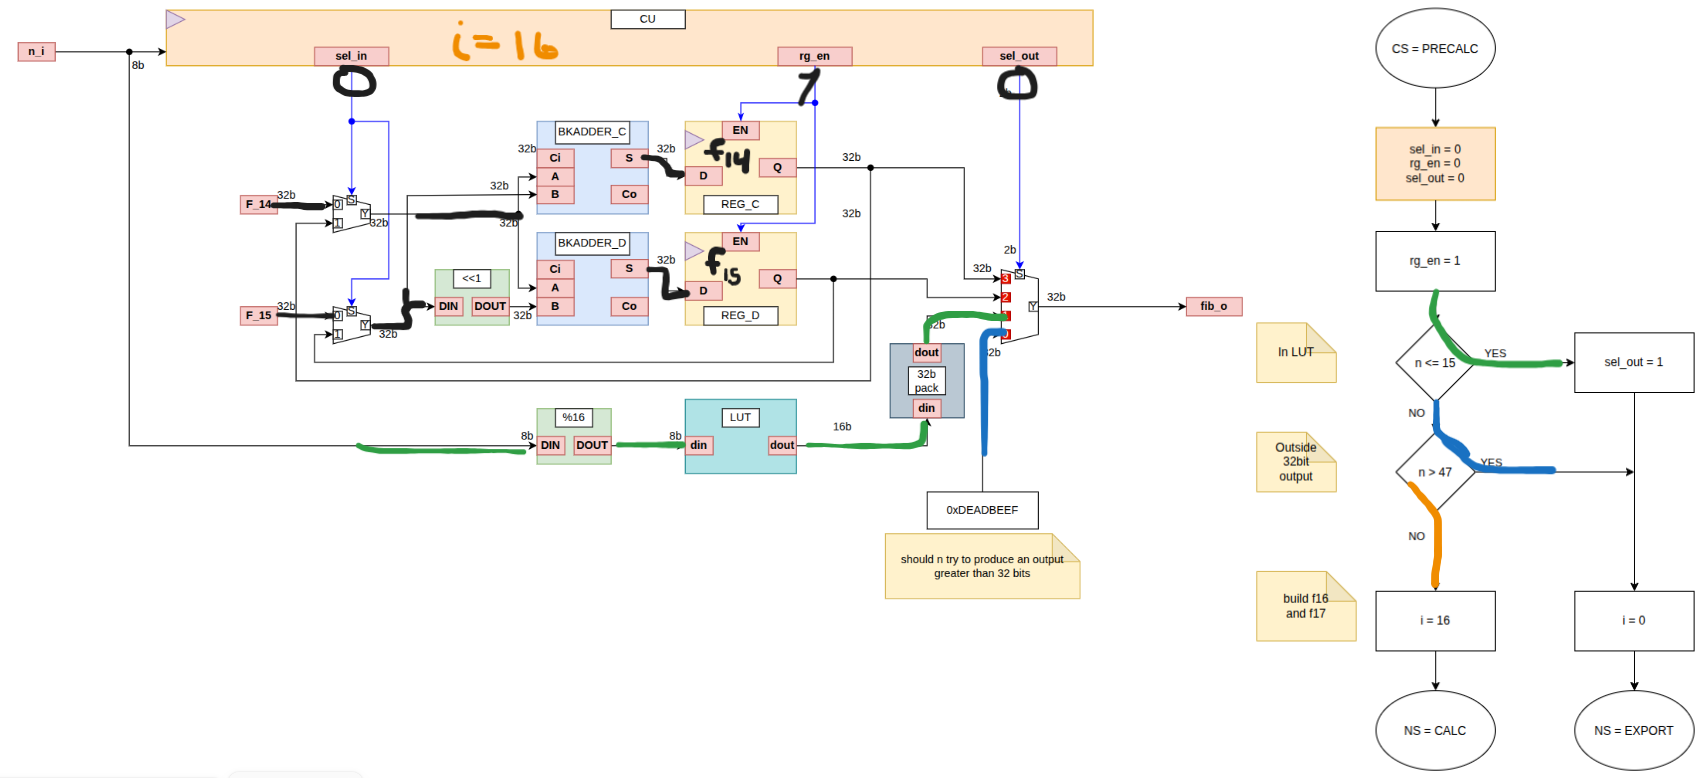
\includegraphics[
						width			= 0.8\textwidth,
						keepaspectratio	= true
					]{./version1/lut_flow.png}
					\caption{\texttt{PRECALC} flow}
					\label{fig:v1-precalc}
				\end{figure}
	
				\begin{figure}[H]
					\centering
					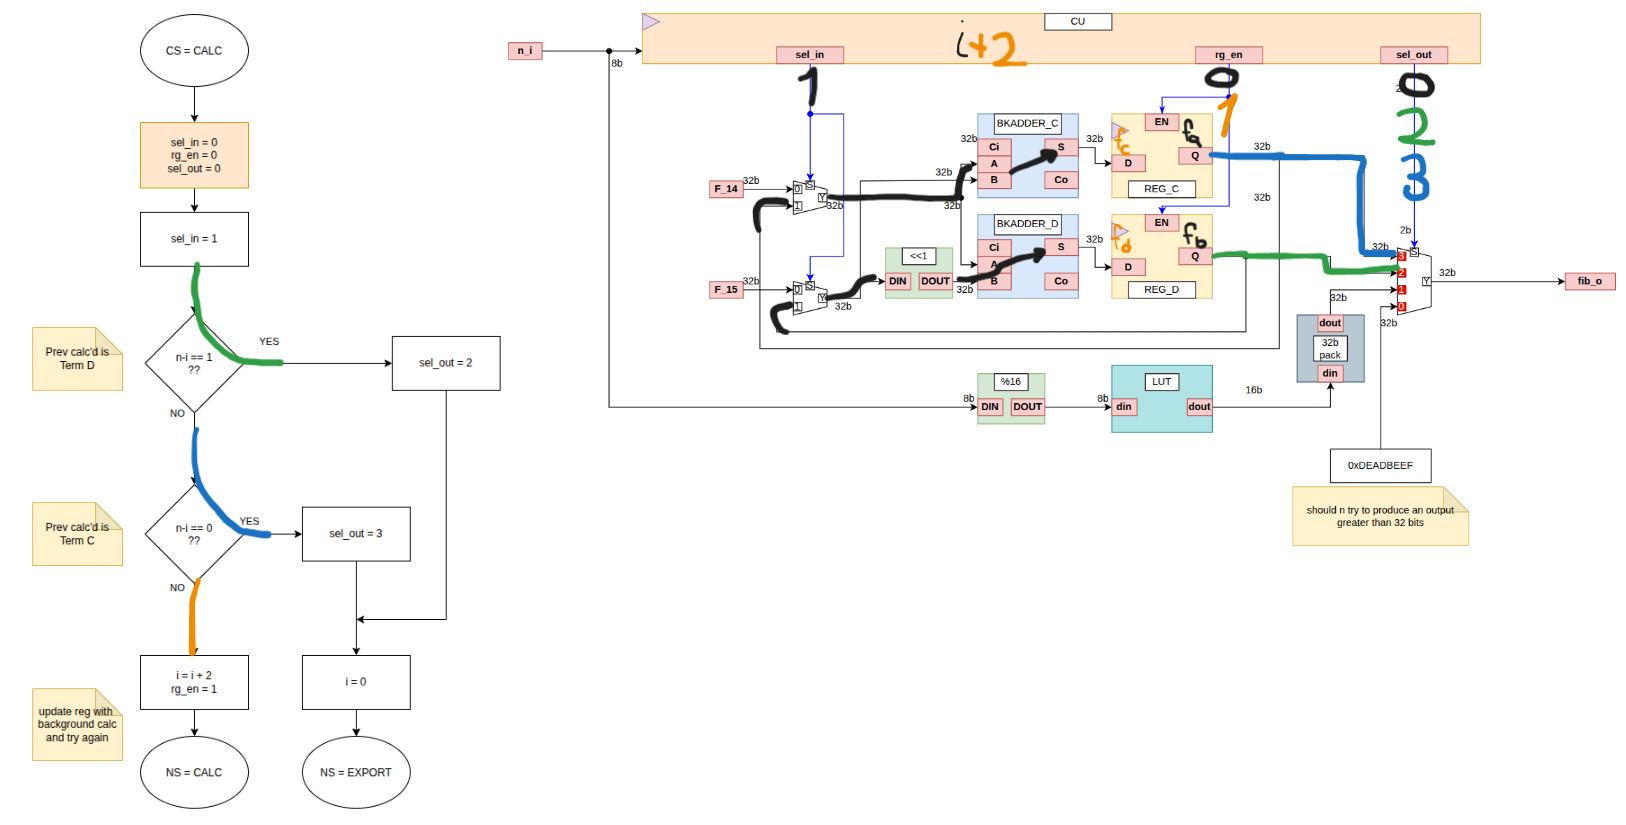
\includegraphics[
						width			= 0.8\textwidth,
						keepaspectratio	= true
					]{./version1/calc_flow.png}
					\caption{\texttt{CALC} flow}
					\label{fig:v1-calc}
				\end{figure}

				Note, the design meets all testing performed on v0. 

				\newpage
				\section{v1 Post-Synthesis Analysis}

					\lstinputlisting[
						basicstyle	= \ttfamily\tiny,
						captionpos	= top,
						caption		= {v1 Pre-PNR Summary},
						breaklines	= false, 
						linerange	= {242-254, 291-305},
						label		= {sta:v1-pre-macro},
					]{./version1/pre_clk_change_overall.log}

					\lstinputlisting[
						basicstyle	= \ttfamily\tiny,
						captionpos	= top,
						caption		= {v1 Pre-PNR STA Highlight},
						breaklines	= false, 
						label		= {sta:v1-pre-summ},
					]{./version1/pre_clk_change_summary.log}

					Fig~\ref{sta:v1-pre-macro} states that we don't have setup 
					or hold violations but fig~\ref{sta:v1-pre-summ} does still
					indicate a few hiccups, having negative slack in our 
					slowest corner case. We've managed to reduce our biggest 
					setup violation by more than a full clock cycle and 
					fanout in fig~\ref{sta:v1-prepnr-long} looks better 
					as well, reducing 126 down to 16! Looking at our critical 
					path, most of our delay is accumulated around driving 
					the output signal \verb|fib_o| as well as \verb|mux_a|. 

					\newpage
					\lstinputlisting[
						basicstyle	=\ttfamily\tiny,
						captionpos	= top,
						caption		= {v1 Pre-PNR Biggest Setup Violator},
						breaklines	= false, 
						firstline	= 5,
						lastline	= 93,
						label		= {sta:v1-prepnr-long}
					]{./version1/pre_clk_change_max.log}

					From here, the easier solutions have been implemented, 
					leaving only a few niche cuts and tunings available. 
					Consider:
					\begin{itemize}
						\item \textbf{Manually reducing the time-padding constants}
							built into librelane/sky130, meeting STA in a naive 
							fashion. This won't improve the logic, just lower
							the timing standards. Different chip makers might
							afford this to the design but it's unlikely 
							(and ultimately not a good idea at this phase 
							of the design). 

						\item \textbf{Further analyze for improvement} will 
							require more time, something is short supply 
							for this project. Entertaining ideas s.a.\ adopting a unique 
							configuration for the muxes, which appear to be
							a constant in our critical path, appear to have 
							merit but are no longer free lunches. Further 
							analysis will have to be performed. 

						\item \textbf{Increasing the clock period} was ultimately
							the option implemented to meet timing - by increasing the period, 
							we preserve our current logic and the sky130A standard
							by making our logic slightly slower.
					\end{itemize}

				\newpage
				\section{v1 meeting STA}

					\lstinputlisting[
						captionpos	= top,
						caption		= {v1's New config file},
						breaklines	= false, 
						label		= {sta:v1-config}
					]{./version1/new_config.yaml}

					\hl{This change will slow the clock from 100MHz to 66MHz.}

					\lstinputlisting[
						basicstyle	= \ttfamily\tiny,
						captionpos	= top,
						caption		= {v1 Post-PNR Summary},
						breaklines	= false, 
						linerange	= {242-254, 291-302},
						label		= {sta:v1-post-macro},
					]{./version1/post_clk_change_overall.log}

					\lstinputlisting[
						basicstyle	= \ttfamily\tiny,
						captionpos	= top,
						caption		= {v1 Post-PNR STA Highlight w/ Clock Change},
						breaklines	= false, 
						label		= {sta:v1-post-sum},
					]{./version1/post_clk_change_summary.log}

					\newpage
					\lstinputlisting[
						basicstyle	=\ttfamily\tiny,
						captionpos	= top,
						caption		= {v1 Post-PNR Biggest Setup Violator w/ Clock Change},
						breaklines	= false, 
						firstline	= 5,
						lastline	= 96,
						label		= {sta:v1-postpnr-long}
					]{./version1/post_clk_change_max.log}

					We've arrived to a point where we don't have setup or
					hold violations nor do we have negative slack across the
					board, seen in fig~\ref{sta:v1-postpnr-long}. There are still
					slew timing violations but they are not as severe as the
					others. By slowing down the clock, we've chosen to make our
					accelerator more conservative and accept the critical path
					in its current state. 

			\chapter{Tile Area}
				The final part of this project was to see if we could
				fit it on a TinyTapeout tile of $160\mu m \times 100\mu m = 16000\mu m^2$. 
				The calculated die area ended up being $20,762\mu m^2$, resulting
				in a  $\sim30\%$ overcast of TT's tile. Potential options for
				shrinking the accelerator could entail:
				 \begin{itemize}
					\item Limiting the output range of our module to 16 or 8 bits.
					\item Storing less numbers in the LUT at the cost of more compute time.
				\end{itemize}

	\chapter{Appendix}
		\section{Code}
			\subsection{RTL}
				
				\lstinputlisting[
					language 	= {Verilog},
					captionpos	= top, 
					caption		= {Mux},
					breaklines	= false, 
					label		= {mux}
				]{../../rtl/Mux_N.sv}

				\lstinputlisting[
					language 	= {Verilog},
					captionpos	= top, 
					caption		= {Brent-Kung `Parallel Prefix' Adder},
					breaklines	= false, 
					label		= {adder}
				]{../../rtl/BKAdder.sv}

				\lstinputlisting[
					language 	= {Verilog},
					captionpos	= top, 
					caption		= {Fibonacci Accelerator},
					breaklines	= false, 
					label		= {fib}
				]{../../rtl/fib.sv}

			\subsection{Simulation SVA Testing}

				\lstinputlisting[
					language 	= {Verilog},
					captionpos	= top, 
					caption		= {Testbench simulation for Fibonacci Accelerator},
					breaklines	= false, 
					label		= {tb-fib}
				]{../../tests/tb_fib/tb_fib.sv}


	\chapter{References}
		\begin{enumerate}
			\item \href{https://github.com/Cal-Poly-Open-Source-ASIC-Class}{CPE490 - OpenSource ASIC}
		\end{enumerate}
		
\end{document}
